\documentclass[en,black,normal,10pt]{elegantnote}
\usepackage{lipsum} % Required for generating dummy text
\usepackage{tikz}
\usetikzlibrary{bayesnet}
\usetikzlibrary{positioning}
\usepackage{caption}
\usepackage{booktabs}
\usepackage{float}
\usepackage{amsmath}

\usetikzlibrary{trees,matrix,arrows,positioning}

\setlength{\parindent}{0pt}

\title{DSAA 5002 - HW2}

%\version{Fall Semester 2023}

\author{50015976 Ruiming ZHANG}
%\institute{Elegant\LaTeX{} Program}

\date{}

\usetikzlibrary{shapes,arrows}

\begin{document}

\maketitle
% logo
%\centerline{\includegraphics[width=0.2\textwidth]{logo-blue}}

\section*{Q1 [25 Marks]}

Consider the following training data with labels 0 and 1, and three
attributes A, B, and C

\definecolor{Gray}{gray}{0.85} % Define a custom color

\begin{table}[H]
    \centering
    \begin{tabular}{ccccc}
        \hline
        \addlinespace[-0.5ex] % 调整间距 \toprule
        \hline
        id & A & B & C & class \\
        \hline
        1 & 0.62 & yes & yes & 0 \\
        \hline
        2 & 3.84 & no & no & 0 \\
        \hline
        3 & 6.61 & yes & no & 0 \\
        \hline
        4 & 6.87 & yes & no & 0 \\
        \hline
        5 & 7.71 & no & yes & 0 \\
        \hline
        6 & 8.98 & no & yes & 0 \\
        \hline
        7 & 1.77 & yes & no & 0 \\
        \hline
        8 & 2.02 & yes & no & 1 \\
        \hline
        9 & 2.06 & no & yes & 1 \\
        \hline
        10 & 2.66 & no & yes & 1 \\
        \hline
        11 & 3.72 & no & yes & 1 \\
        \hline
        12 & 4.98 & yes & yes & 1 \\
        \hline
        13 & 5.73 & yes & yes & 1 \\
        \hline
        14 & 6.29 & yes & yes & 1 \\
        \hline
        15 & 9.08 & no & no & 1 \\
        \hline
        16 & 9.45 & no & no & 1 \\
        \hline
        \addlinespace[-0.5ex] % 调整间距 \toprule
        \hline
    \end{tabular}
\end{table}

\begin{itemize}
    \item[(a)] (10 marks) Try threshold 2, 5, and 8 for attributes A (that is, use the “A > 2, A < 2”, “A > 5, A < 5”, and “A > 8, A < 8” respectively). Use the Gini score to determine the best one $\theta_a$ among them. Recall:
    \begin{equation*}
        Gini(t) = 1 - \sum_{i = 1}^{c} [p(i|t)]^2  
    \end{equation*}
    \item[(b)] (20 marks) Use $\theta_a$ obtained above, and the Gini score, determine which attributes should firstly be used for developing a decision tree.
\end{itemize}

\subsection*{Solution:}

\paragraph*{(a)} We have: $Info(T) = 1 - (\frac{7}{16})^2 - (\frac{9}{16})^2 = \frac{63}{128} \approx 0.4922$

For threshold 2:

$Info(T_{A<2}) = 1 - \frac{2}{2}^2 - \frac{0}{2}^2 = 0$

$Info(T_{A>2}) = 1 - \frac{5}{14}^2- \frac{9}{14}^2 = \frac{45}{98} \approx 0.4592$

$Info(A_{threshold=2}, T) = \frac{2}{16} \times 0 + \frac{14}{16} \times \frac{45}{98} = \frac{45}{122} \approx 0.4018$

$Gain(A_{threshold=2}, T) = \frac{63}{128} - \frac{45}{122} = \frac{81}{896} \approx 0.0904$

For threshold 5:

$Info(T_{A<5}) = 1 - \frac{3}{8}^2 - \frac{5}{8}^2 = \frac{15}{32} \approx 0.4688$

$Info(T_{A>5}) = 1 - \frac{4}{8}^2- \frac{4}{8}^2 = 0.5$

$Info(A_{threshold=5}, T) = \frac{8}{16} \times \frac{15}{32} + \frac{8}{16} \times \frac{1}{2} = \frac{31}{64} \approx 0.4844$

$Gain(A_{threshold=5}, T) = \frac{63}{128} - \frac{31}{64} = \frac{1}{128} \approx 0.0078$

For threshold 8:

$Info(T_{A<8}) = 1 - \frac{6}{13}^2 - \frac{7}{13}^2 = \frac{84}{169} \approx 0.4970$

$Info(T_{A>8}) = 1 - \frac{1}{3}^2- \frac{2}{3}^2 = \frac{4}{9} \approx 0.4444$

$Info(A_{threshold=8}, T) = \frac{13}{16} \times \frac{84}{169} + \frac{3}{16} \times \frac{4}{9} = \frac{19}{39} \approx 0.4872$

$Gain(A_{threshold=8}, T) = \frac{63}{128} - \frac{45}{122} = \frac{81}{896} \approx 0.0050$

Hence, the best $\theta_a$ is 2.

\paragraph*{(b)}

For attribute B:

$Info(T_{B=yes}) = 1 - \frac{4}{8}^2 - \frac{4}{8}^2 = 0.5$

$Info(T_{B=no}) = 1 - \frac{3}{8}^2- \frac{5}{8}^2 = \frac{15}{32} \approx 0.4688$

$Info(B, T) = \frac{8}{16} \times \frac{1}{2} + \frac{8}{16} \times \frac{15}{32} = \frac{31}{64} \approx 0.4844$

$Gain(B, T) = \frac{63}{128} - \frac{31}{64} = \frac{1}{128} \approx 0.0078$

For attribute C:

$Info(T_{C=yes}) = 1 - \frac{3}{9}^2 - \frac{6}{9}^2 = \frac{4}{9} \approx 0.4444$

$Info(T_{C=no}) = 1 - \frac{4}{7}^2- \frac{3}{7}^2 = \frac{4}{9} \approx 0.4898$

$Info(C, T) = \frac{9}{16} \times \frac{84}{169} + \frac{7}{16} \times \frac{4}{9} = \frac{13}{28} \approx 0.4643$

$Gain(C, T) = \frac{63}{128} - \frac{13}{28} = \frac{25}{896} \approx 0.0279$

Hence, the attribute should firstly be used is attribute A.
\section*{Q2 [30 Marks]}

The table below is a small part of the Acute Inflammations Data Set.

\begin{table}[H]
    \begin{tabular}{ll}
        a1 & Temperature of patient (35C-42C) \\
        a2 & Occurrence of nausea (yes, no) \\
        a3 & Lumbar pain (yes, no) \\
        a4 & Urine pushing (continuous need for urination) (yes, no) \\
        a5 & Micturition pains (yes, no) \\
        a6 & Burning of urethra, itch, swelling of urethra outlet (yes, no) \\
        d1 & Decision: Inflammation of urinary bladder (yes, no) \\
        d2 & Decision: Nephritis of renal pelvis origin (yes, no) \\
    \end{tabular}
\end{table}

Here the attributes a1-a6 are observations, and the decisions d1 and d2 are made by a
medical expert. The purpose of studying this data set is to predict presumptive diagnosis
of two disease of the urinary system, namely, “Inflammation of urinary bladder” and
“Nephritis of renal pelvis origin".

\begin{table}[H]
    \centering
    \begin{tabular}{cccccc|cc}
        \hline
        \addlinespace[-0.5ex] % 调整间距 \toprule
        \hline
        a1 & a2 & a3 & a4 & a5 & a6 & d1 & d2 \\
        \hline
        37.3 & no & yes & no & no & no & no & no \\
        \hline
        37.4 & no & no & yes & no & no & yes & no \\
        \hline
        37.5 & yes & yes & no & no & no & no & no \\
        \hline
        37.6 & no & no & yes & yes & yes & yes & yes \\
        \hline
        37.7 & no & no & yes & no & no & yes & no \\
        \hline
        37.7 & no & no & yes & yes & no & yes & no \\
        \hline
        37.7 & no & no & yes & yes & no & yes & no \\
        \hline
        37.8 & no & yes & no & no & no & no & no \\
        \hline
        37.9 & no & no & yes & yes & yes & yes & no \\
        \hline
        37.9 & no & no & yes & no & no & yes & no \\
        \hline
        38.0 & no & yes & yes & no & yes & no & yes \\
        \hline
        38.0 & no & yes & yes & no & yes & no & yes \\
        \hline
        38.1 & no & yes & yes & no & yes & yes & yes \\
        \hline
        38.3 & no & yes & yes & no & yes & no & yes \\
        \hline
        38.5 & no & yes & yes & no & yes & no & no \\
        \hline
        38.7 & no & yes & yes & no & yes & no & yes \\
        \hline
        38.9 & no & yes & yes & no & yes & yes & yes \\
        \hline
        39.0 & no & yes & yes & no & yes & no & yes \\
        \hline
        39.4 & no & yes & yes & no & yes & no & yes \\
        \hline
        39.5 & no & yes & yes & no & yes & no & yes \\
        \hline
        \addlinespace[-0.5ex] % 调整间距 \bottomrule
        \hline
    \end{tabular}
\end{table}

\begin{itemize}
    \item[(a)] (10 marks) Consider the procedures of building a decision tree with Gini score. If we plan only to use the attributes a3 and a5 to predict the decision d2, which attribute should we use first?
    \item[(b)] (20 marks) Use the naïve Bayes algorithm, the attributes a1 (with the threshold $\theta_1$ = 37.95), a2, and a3 only, to predict the decision d2 for the following data of a new patient. (For simplicity you do NOT need to use the Laplacian correction.)
\end{itemize}

\begin{table}[H]
    \centering
    \begin{tabular}{cccccc|cc}
        \hline
        \addlinespace[-0.5ex] % 调整间距 \toprule
        \hline
        a1 & a2 & a3 & a4 & a5 & a6 & d1 & d2 \\
        \hline
        40.0 & yes & no & no & no & no & ? & ? \\
        \hline
        \addlinespace[-0.5ex] % 调整间距 \bottomrule
        \hline
    \end{tabular}
\end{table}

\subsection*{Solution:}

\paragraph*{(a)} Because we only predict the decision d2, we have: $Info(T)=1-\frac{1}{2}^2-\frac{1}{2}^2=0.5$

For attribute a3, we have:

$Info(T_{yes}) = 1 - \frac{9}{13}^2 - \frac{4}{13}^2 = \frac{72}{169} \approx 0.4260$

$Info(T_{no}) = 1 - \frac{1}{7}^2- \frac{6}{7}^2 = \frac{12}{49} \approx 0.2499$

$Info(a3, T) = \frac{13}{20} \times \frac{72}{169} + \frac{7}{20} \times \frac{12}{49} = \frac{33}{91} \approx 0.3626$

$Gain(a3, T) = 0.5 - 0.3626 = 0.1374$

For attribute a5, we have:

$Info(T_{yes}) = 1 - \frac{1}{4}^2 - \frac{3}{4}^2 = \frac{3}{8} = 0.3750$

$Info(T_{no}) = 1 - \frac{9}{16}^2- \frac{7}{16}^2 = \frac{63}{128} \approx 0.4922$

$Info(a5, T) = \frac{4}{20} \times \frac{3}{8} + \frac{16}{20} \times \frac{63}{128} = \frac{15}{32} \approx 0.4688$

$Gain(a5, T) = 0.5 - 0.4688 = 0.0312$

We can see $Gain(a3, T) > Gain(a5, T)$, so we should use a3 first.

\paragraph*{(b)} Because we have:

For attribute a1:

$P(a1>\theta_1|d2=yes)=\frac{9}{10}=0.9$

$P(a1<\theta_1|d2=yes)=\frac{1}{10}=0.1$

$P(a1>\theta_1|d2=no)=\frac{1}{10}=0.1$

$P(a1<\theta_1|d2=no)=\frac{9}{10}=0.9$

For attribute a2:

$P(a2=yes|d2=yes)=\frac{0}{10}=0$

$P(a2=no|d2=yes)=\frac{10}{10}=1$

$P(a2=yes|d2=no)=\frac{1}{10}=0.1$

$P(a2=no|d2=no)=\frac{9}{10}=0.9$

For attribute a3:

$P(a3=yes|d2=yes)=\frac{9}{10}=0.9$

$P(a3=no|d2=yes)=\frac{1}{10}=0.1$

$P(a3=yes|d2=no)=\frac{4}{10}=0.4$

$P(a3=no|d2=no)=\frac{6}{10}=0.6$

Then we have:

{
    \setlength{\abovedisplayskip}{-10pt}
    \setlength{\belowdisplayskip}{0pt}

    \begin{flalign*}
        P &= P(a1>\theta_1,a2=yes,a3=no) && \\
            &= P(a1>\theta_1) \times P(a2=yes)\times P(a3=no) \\
            &=0.00875
    \end{flalign*}

    \begin{flalign*}
        P_1 &= P(a1>\theta_1,a2=yes,a3=no|d2=yes) && \\
            &= P(a1>\theta_1|d2=yes) \times P(a2=yes|d2=yes)\times P(a3=no|d2=yes) \\
            &=0.9 \times 0 \times 0.1 \\
            &=0
    \end{flalign*}

    \begin{flalign*}
        P_2 &= P(a1>\theta_1,a2=yes,a3=no|d2=no) && \\
            &= P(a1>\theta_1|d2=no) \times P(a2=yes|d2=no)\times P(a3=no|d2=no) \\
            &=0.1 \times 0.1 \times 0.6 \\
            &=0.006
    \end{flalign*}
}

Thus: 

{
    \setlength{\abovedisplayskip}{-10pt}
    \setlength{\belowdisplayskip}{0pt}

    \begin{flalign*}
        &P(d2=yes|a1>\theta_1,a2=yes,a3=no) \\
            &=\frac{P_1 \times P(d2=yes)}{P} && \\
            &=\frac{0 \times 0.5}{0.00875} \\
            &=0
    \end{flalign*}

    \begin{flalign*}
        &P(d2=no|a1>\theta_1,a2=yes,a3=no) \\
            &=\frac{P_2 \times P(d2=no)}{P} && \\
            &=\frac{0.006 \times 0.5}{0.00875} \\
            &=0.3429
    \end{flalign*}
}

Hence, the decision of d2 is no.
\section*{Q3 [15 Marks]}

There is a BBN below, which comprises four Random Variables(RV).
Each RV is a Boolean RV

\begin{center}
    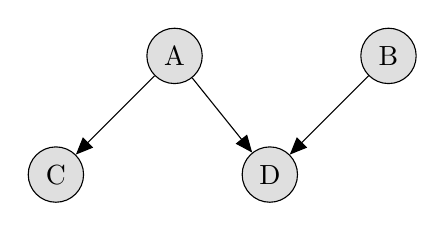
\begin{tikzpicture}
        % Define nodes
        \node[obs] (A) {A};
        \node[obs, right=2cm of A] (B) {B};
        \node[obs, below left=1cm and 1cm of A] (C) {C};
        \node[obs, right=2cm of C] (D) {D};
        % Connect nodes
        \edge {A} {C};
        \edge {A,B} {D};
    \end{tikzpicture}
\end{center}

\begin{table}[H]
    \centering
    \begin{tabular}{lll}
        \(P(A) = 0.1\) & \(P(B) = 0.5\) & \(P(C|A) = 0.7\) \\
        \(P(C|\lnot A) = 0.2\) & \(P(D|A, B) = 0.9\) & \(P(D|\lnot A, B) = 0.6\) \\
        \(P(D|A, \lnot B) = 0.7\) & \(P(D|\lnot A, \lnot B) = 0.3\)
    \end{tabular}
\end{table}

\begin{itemize}
    \item[(a)] (7 marks) What is $P(\lnot A, B, \lnot C, D)$?
    \item[(b)] (8 marks) What is $P(A | B, C, D)$?
\end{itemize}

\subsection*{Solution:}

\paragraph*{(a)} According to the BBN above, we have:

{
    \setlength{\abovedisplayskip}{-10pt}
    \setlength{\belowdisplayskip}{0pt}

    \begin{flalign*}
        P(\lnot A, B, \lnot C, D) &= P(B, D|\lnot A, \lnot C) \times P(\lnot A, \lnot C)&& \\
            &= P(B, D | \lnot A) \times P(\lnot C | \lnot A) \times P(\lnot A) && \\
            &= P(D|\lnot A B) \times P(B) \times [1 - P(C | \lnot A)] \times [1 - P(A)] && \\
            &= 0.6 \times 0.5 \times (1-0.2) \times (1-0.1) && \\
            &= 0.216
    \end{flalign*}
}

\paragraph*{(b)} According to the BBN above, we have:

{
    \setlength{\abovedisplayskip}{-10pt}
    \setlength{\belowdisplayskip}{0pt}

    \begin{flalign*}
        P(A | B, C, D) &= \frac{P(A, B, C, D)}{P(B, C, D)} && \\
            &= \frac{P(B, D | A, C) \times P(A, C)}{P(B, C, D)} && \\
            &= \frac{P(B, D | A) \times P(A, C)}{P(B, D) \times P(C)} && \\
            &= \frac{P(D | A, B) \times P(B) \times [P(C | A) \times P(A)]}{[P(B, D, A) + P(B, D, \lnot A)] \times P(C)} && \\
            &= \frac{P(D | A, B) \times P(B) \times [P(C | A) \times P(A)]}{[P(D | A, B) \times P(A, B) + P(D | \lnot A, B) \times P(\lnot A, B)] \times P(C)} && \\
        \end{flalign*}
}

Except for \( P(C) \), all other variables are known. According to Total Probability Formula, we have:

{
    \setlength{\abovedisplayskip}{-10pt}
    \setlength{\belowdisplayskip}{0pt}

    \begin{flalign*}
        P(C) &= P(C, A) + P(C, \lnot A) && \\
            &= P(C | A) \times P(A) + P(C | \lnot A) \times P(\lnot A) && \\
            &= 0.7 \times 0.1 + 0.2 \times 0.9 && \\
            &= 0.25
    \end{flalign*}
}

Hence:

$P(A | B, C, D) = \frac{0.9 \times 0.5 \times [0.7 \times 0.1]}{[0.9 \times 0.1 \times 0.5 + 0.6 \times 0.9 \times 0.5] \times 0.25} = 0.4$
\section*{Q4 [20 Marks] Fuzzy Cluster} 

Assume there are 2 clusters in which the data is to be divided, initializing the data point randomly. 
Each data point lies in both clusters with some membership value which can be assumed anything in the initial state.
The table below represents the values of the data points along with their membership (gamma) in each cluster.

\begin{table}[h]
    \centering
    \begin{tabular}{|c|c|c|c|c|c|}
    \hline
    Cluster & (1,3) & (2,5) & (4,8) & (7,9) & (9,12) \\
    \hline
    1)      & 0.8   & 0.7   & 0.5   & 0.3   & 0.1    \\
    \hline
    2)      & 0.2   & 0.3   & 0.5   & 0.7   & 0.9    \\
    \hline
    \end{tabular}
\end{table}

Please work out the centroids, the distance of each point from centroid, and the cluster membership value.

\subsection*{Solution:}

About the Fuzzy Clustering Using the EM Algorithm, we have the following formula:\\
E step:

\[
    W_{i1} = \frac{\frac{1}{\text{dist}(o_i, c_1)^2}}{\left( \frac{1}{\text{dist}(o_i, c_1)^2} + \frac{1}{\text{dist}(o_i, c_2)^2} \right)}
    = \frac{\text{dist}(o_i, c_2)^2}{\text{dist}(o_i, c_2)^2 + \text{dist}(o_i, c_1)^2}
\]

\[
    W_{i2} = \frac{\frac{1}{\text{dist}(o_i, c_2)^2}}{\left( \frac{1}{\text{dist}(o_i, c_1)^2} + \frac{1}{\text{dist}(o_i, c_2)^2} \right)}
    = \frac{\text{dist}(o_i, c_1)^2}{\text{dist}(o_i, c_2)^2 + \text{dist}(o_i, c_1)^2}
    = 1-W_{i1}
\]

M step:

\[
    c_1 = \left( 
    \frac{\sum_\text{each point o} (w_{o,c_1}^2 * o_x)}{\sum_\text{each point o} w_{o,c_1}^2}, 
    \frac{\sum_\text{each point o} (w_{o,c_1}^2 * o_y)}{\sum_\text{each point o} w_{o,c_1}^2} 
    \right)
\]

\[
    c_2 = \left( 
    \frac{\sum_\text{each point o} (w_{o,c_2}^2 * o_x)}{\sum_\text{each point o} w_{o,c_2}^2}, 
    \frac{\sum_\text{each point o} (w_{o,c_2}^2 * o_y)}{\sum_\text{each point o} w_{o,c_2}^2} 
    \right)
\]

\textbf{Iteration 1}: \\
According to the table below, we already have the result of E step: 

\[
    M^T =
    \begin{bmatrix}
        0.8 & 0.7 & 0.5 & 0.3 & 0.1 \\
        0.2 & 0.3 & 0.5 & 0.7 & 0.9 \\
    \end{bmatrix}
\]

Then we have the M step:

\[
    c_1 = \left( 
        \frac{0.8^2*1+0.7^2*2+0.5^2*4+0.3^2*7+0.1^2*9}{0.8^2+0.7^2+0.5^2+0.3^2+0.1^2}, 
        \frac{0.8^2*3+0.7^2*5+0.5^2*8+0.3^2*9+0.1^2*12}{0.8^2+0.7^2+0.5^2+0.3^2+0.1^2} 
        \right)
\]

\[
    c_2 = \left( 
        \frac{0.2^2*1+0.3^2*2+0.5^2*4+0.7^2*7+0.9^2*9}{0.2^2+0.3^2+0.5^2+0.7^2+0.9^2}, 
        \frac{0.2^2*3+0.3^2*5+0.5^2*8+0.7^2*9+0.9^2*12}{0.2^2+0.3^2+0.5^2+0.7^2+0.9^2} 
        \right)
\]

Then we have $c_1 = (2.2568, 4.9324)$ and $c_2 = (7.1071, 9.9405)$.

\textbf{Iteration 2}: \\
E step: \\
Here we just calculate point d = (1,3) as an example: \\
First calculate the distance between the point and the centroids. \\
To simplify the calculation, we just calculate the square of the distance.

\[
    dist_sq((1,3), c_1) = (1-2.2568)^2 + (3-4.9324)^2 = 5.3137
\]

\[
    dist_sq((1,3), c_2) = (1-7.1071)^2 + (3-9.9405)^2 = 85.4672
\]

Then we have the result of E step:

\[
    w_{d,c_1} = \frac{85.4672}{85.4672+5.3137} = 0.9415
\]

\[
    w_{d,c_2} = 1 - w_{d,c_1} = 0.0585
\]

The rest of the calculation is similar to the first iteration. Then we have the result of M step:

\begin{table}[h]
    \centering
    \begin{tabular}{|c|c|c|c|c|c|}
    \hline
    Cluster & (1,3) & (2,5) & (4,8) & (7,9) & (9,12) \\
    \hline
    1)      & 0.9415   & 0.9986   & 0.5188   & 0.0224   & 0.0758    \\
    \hline
    2)      & 0.0585   & 0.0014   & 0.4812   & 0.9776   & 0.9242    \\
    \hline
    \end{tabular}
\end{table}

M step:

Similar to the first iteration, we have the result of M step:
we have $c_1 = (1.8585, 4.5724)$ and $c_2 = (7.4856, 10.1299)$.

\textbf{Iteration 3}: \\
Similar to the second iteration, just show the full result of E step and M step:

\begin{table}[h]
    \centering
    \begin{tabular}{|c|c|c|c|c|c|c|c|}
    \hline
    Cluster & (1,3) & (2,5) & (4,8) & (7,9) & (9,12) & $c_x$ & $c_y$    \\
    \hline
    1)      & 0.9666   & 0.9964   & 0.5053   & 0.0318   & 0.0517 & 1.8171 & 4.5061  \\
    \hline
    2)      & 0.0334   & 0.0036   & 0.4947   & 0.9682   & 0.9483 & 7.5079 & 10.1747  \\
    \hline
    \end{tabular}
\end{table}

I have put the entire calculation process in the attachment of this homework, a .ipynb file.

\end{document}
